%%%%%%%%%%%%%%%%%%%%%%%%%%%%%%%%%%%%%%%%%%%%%%%%%%%%%
%%% Task 4 %%%%%%%%%%%%%%%%%%%%%%%%%%%%%%%%%%%%%%%%%%
%%%%%%%%%%%%%%%%%%%%%%%%%%%%%%%%%%%%%%%%%%%%%%%%%%%%%
\task{Synchronous generator}

\taskGerman{Synchrongenerator}

An externally excited synchronous generator is directly fed from a wind turbine without utilizing a gear.
For the three-phase generator the parameters from \autoref{tab:para_SynchonousMachine} are known.

\vspace{1em}
\color{gray}
Ein elektrisch erregter Synchrongenerator wird von einer Windturbine direkt angetrieben (getriebeloser Windgenerator). Für den Drehstromgenerator sind die Parameter aus \autoref{tab:para_SynchonousMachine} bekannt.
\color{black}

\begin{table}[htb]
    \caption{Parameters of the synchronous generator.}
    \centering
    \begin{tabular}{llll}\toprule
    Symbol       & Value    & Symbol    & Value \\
    \midrule
    $P_{\mathrm{n,el}}$    & $\SI{-1.5}{\mega\watt}$ & $l_{\mathrm{z}}$   & $\SI{700}{\milli\metre}$ \\
    $d_{\mathrm{s}}$       & $\SI{5}{\metre}$       & $n_{\mathrm{n}}$    & $\SI{15}{\per\minute}$ \\
    $N_{\mathrm{w}}$       & 3 windings per coil    & $q$    & 2 \\
    $2p$                   & 90                     & $\frac{y}{\rho_{\mathrm{p}}}$    & $\frac{5}{6}$ \\
    \bottomrule
    \end{tabular}
    \label{tab:para_SynchonousMachine}
\end{table}
\vspace{-1.3em}
 \subtask{Calculate the nominal torque $T_{\mathrm{n}}$ at the rated conditions of the generator. At this operating point, the efficiency is given with $\eta_{\mathrm{n}}$ = 95 \%.}{2}
\subtaskGerman{Berechne das Nenndrehmoment $T_{\mathrm{n}}$ im Nennarbeitspunkt. In diesem Arbeitspunkt ist der \\ Wirkungsgrad mit $\eta_{\mathrm{n}}$ = 95 \% gegeben. }

\begin{solutionblock}
    In the task, only the electrical power is given, therefore, calculating the mechanical power by
    $$ P_{\mathrm{n,mech}} = \frac{P_{\mathrm{n,el}}}{\eta_{\mathrm{n}}} = \frac{\SI{-1.5}{\mega\watt}}{0.95} = \SI{-1.578947}{\mega\watt}$$
    
    and the torque at the nominal operating is determined as:
    $$ T_{\mathrm{n}} = \frac{P_{\mathrm{n,mech}}}{\omega_{\mathrm{n}}} = \frac{\SI{-1.578947}{\mega\watt}}{2\pi \cdot \SI{0.25}{\per\second}} = \SI{-1005.189}{\kilo\newton\metre}.$$
\end{solutionblock}

\subtask{How large is the number of winding turns per phase $N_{\mathrm{w,phase}}$, when the total 90 coils are parallelized in 5 groups?}{1}
\subtaskGerman{Wie groß ist die Windungszahl pro Phase $N_{\mathrm{w,phase}}$ bei Parallelschaltung der insgesammt 90 Spulen in 5 Gruppen?}

\begin{solutionblock}
    The number of winding turns per phase is: 
    $$
    N_{\mathrm{w,phase}} = \frac{2p q N_{\mathrm{w}}}{a} = \frac{90 \cdot 2 \cdot 3}{5} = 108.
    $$
\end{solutionblock}


\subtask{Calculate the winding factor $\zeta_{\mathrm{w,}k}$ for the fundamental wave ($k$ = 1).}{2}
\subtaskGerman{Berechne den Wicklungsfaktor $\zeta_{\mathrm{w,}k}$ für die Grundwelle ($k$ = 1).}

\begin{solutionblock}
    The winding factor is defined by
    $$ \zeta_{\mathrm{w,}k} = \zeta_{\mathrm{d,}k} \zeta_{\mathrm{p,}k}, $$
    where $\zeta_{\mathrm{d,}k}$ represents the distribution and $\zeta_{\mathrm{p,}k}$ the pitch factor.
    With $m$ = 3 phases, the distribution factor calculates as
    $$\zeta_{\mathrm{d,}1} = \frac{\sin\left(\frac{\pi}{2m} \right)}{q\sin\left(\frac{\pi}{2mq} \right)} 
    = \frac{\sin\left(\frac{\pi}{2\cdot3}\right)}{2 \cdot \sin\left(\frac{\pi}{2\cdot3\cdot 2} \right)}
    = 0.966,
    $$
    and, the pitch factor is determined with
    $$
    \zeta_{\mathrm{p,}1} = \sin\left(\frac{\pi}{2} \frac{y}{\rho_{\mathrm{p}}}\right)
    = \sin\left(\frac{\pi}{2} \cdot \frac{5}{6} \right) = 0.966,
    $$
    which results in the winding factor by
    $$ \zeta_{\mathrm{w,}1} =  \zeta_{\mathrm{d,}1}  \zeta_{\mathrm{p,}1} = 0.966 \cdot 0.966 = 0.933. $$
    
\end{solutionblock}


\subtask{The flux density of the fundamental wave of one phase is given with $\hat{B}_{\updelta}^{(1)} = \SI{1}{\tesla}$. Determine at nominal speed $n_{\mathrm{n}}$ the flux per pole $\phi_{\updelta}$ and the induced voltage per phase $U_{\mathrm{i,phase}}$.}{2}
\subtaskGerman{Die Grundwelle der Flussdichte für eine Phase ist gegeben mit $\hat{B}_{\updelta}^{(1)} = \SI{1}{\tesla}$. Bestimmen Sie den Fluss pro Pol $\phi_{\updelta}$ und die induzierte Spannung pro Phase $U_{\mathrm{i,phase}}$ bei der nominellen Drehzahl.}


\begin{solutionblock}
    The pole pitch as a distance in meter is calculated by
    $$ \tau_{\mathrm{p}} = \frac{d_{\mathrm{si}} \pi}{2p} = \frac{\SI{5}{\metre}\cdot \pi}{90} = \SI{0.1745}{\metre},$$

    and the effective cross-sectional area of the machine per pole is determined with
    $$ A_{\updelta} = \tau_{\mathrm{p}} l_{\mathrm{z}} = \SI{0.1745}{\metre} \cdot \SI{0.7}{\metre}
    = \SI{0.122}{\metre^2}.$$

    Hence, the air gap flux is given with
    $$ \phi_{\updelta} = A_{\updelta} \hat{B}_{\updelta}^{(1)} = \SI{0.122}{\metre^2} \cdot \SI{1}{\tesla} = \SI{0.122}{\volt\second},$$

    the electrical angular frequency is determined by
    $$ \omega_{\mathrm{el}} = 2 \pi f_{\mathrm{mech}} p = 2 \pi \cdot \SI{0.25}{\per\second} \cdot 45 = \SI{70.69}{\per\second}$$

    resulting in the induced voltage of 
    $$ U_{\mathrm{i,phase}} = \omega_{\mathrm{el}} N_{\mathrm{w,phase}} \zeta_{\mathrm{w,}1} \phi_{\updelta} = \SI{70.69}{\per\second} \cdot 108 \cdot 0.933 \cdot \SI{0.122}{\volt\second} = \SI{869}{\volt}. $$
    
\end{solutionblock}




\subtask{Assume that the flux density in the air gap is a superposition of sine waves. Draw the trajectories of the flux densities $B_{\updelta}^{(1)}(\vartheta)$ and $B_{\updelta}^{(3)}(\vartheta)$ for one phase in the template (\autoref{fig:B_sketch_fund}).}{2}

\subtaskGerman{Nehmen Sie an, dass die Flussdichte im Luftspalt eine Überlagerung von Sinuswellen darstellt. Zeichnen Sie die Trajektorien der Flussdichten $B_{\updelta}^{(1)}(\vartheta)$ und $B_{\updelta}^{(3)}(\vartheta)$ für eine Phase in die \autoref{fig:B_sketch_fund}.}
\begin{figure}[ht!]
    \centering
    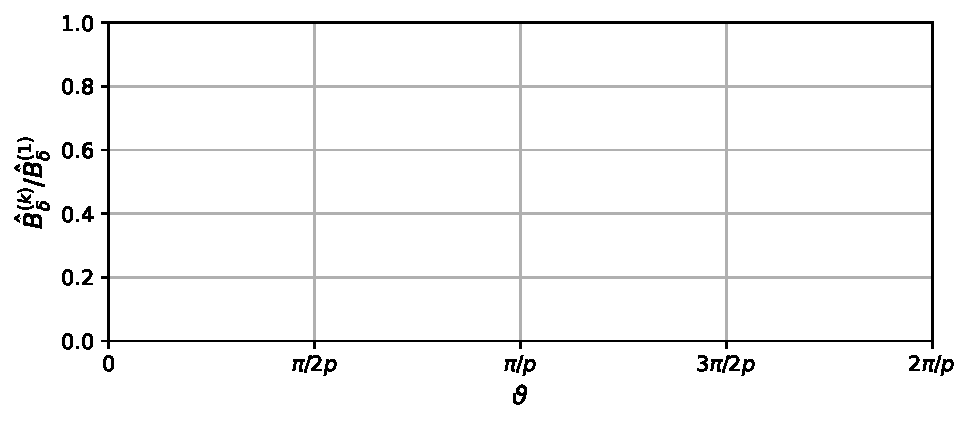
\includegraphics{fig/B_sketch_fund.pdf}
    \caption{Template to draw the flux densities over the stator circumference $\vartheta$.}
    \label{fig:B_sketch_fund}
\end{figure}%

\begin{solutionblock}
    The distribution factor for the third harmonic ($k$ = 3) calculates as
    $$\zeta_{\mathrm{d,}3} = \frac{\sin\left(\frac{3\pi}{2m} \right)}{q\sin\left(\frac{3\pi}{2mq} \right)} 
    = \frac{\sin\left(\frac{3\cdot \pi}{2\cdot3}\right)}{2 \cdot \sin\left(\frac{3\cdot \pi}{2\cdot3\cdot 2} \right)}
    = 0.707,
    $$
    and, the pitch factor is determined with
    $$
    \zeta_{\mathrm{p,}3} = \sin\left(3 \cdot \frac{\pi}{2} \frac{y}{\rho_{\mathrm{p}}}\right)
    = \sin\left(3 \cdot \frac{\pi}{2} \cdot \frac{5}{6} \right) = -0.707,
    $$
    which results in the winding factor by
    $$ \zeta_{\mathrm{w,}3} =  \zeta_{\mathrm{d,}3}  \zeta_{\mathrm{p,}3} = 0.707 \cdot -0.707 = -0.500. $$

    The winding factor must set into the relationship of the fundamental wave by
    $$ \frac{B_{\updelta}^{(3)}(\vartheta)}{B_{\updelta}^{(1)}(\vartheta)} = \frac{-0.5}{0.933} = -0.54, $$
    which is the amplitude for the third harmonic. Both trajectories are shown in \autoref{fig:sol_B_sketch_fund}.

    \begin{solutionfigure}[ht!]
    \centering
    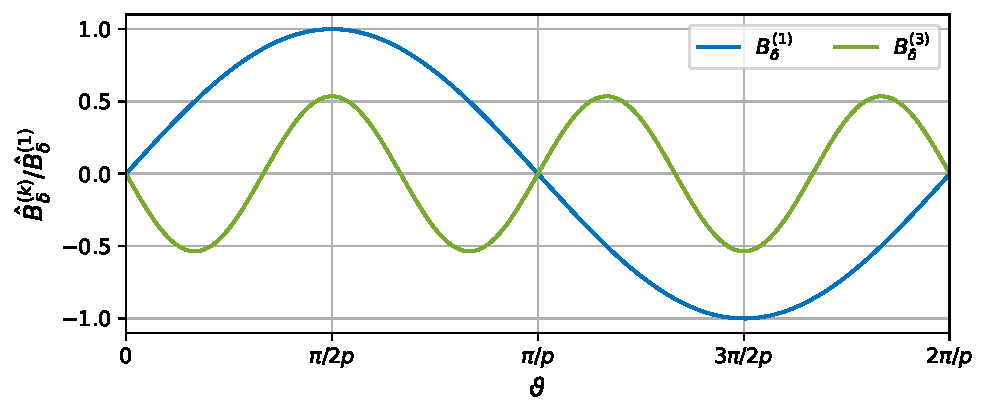
\includegraphics{fig/sol_B_sketch_fund.pdf}
    \caption{Solution trajectories for $B_{\updelta}^{(1)}(\vartheta)$ and $B_{\updelta}^{(3)}(\vartheta)$.}
    \label{fig:sol_B_sketch_fund}
    \end{solutionfigure}
\end{solutionblock}


\subtask{Is the third harmonic ($k$ = 3) problematic for this type of machine?}{1}
\subtaskGerman{Ist die dritte Harmonische ($k$ = 3) für diesen Maschinentyp problematisch?}

\begin{solutionblock}
    Due to the three-phase winding system of this machine, the third harmonic is canceled out and, therefore, no problem occurs.
\end{solutionblock}


\subtask{Is it possible to connect the wind turbine directly to the grid?}{1}
\subtaskGerman{Kann der Synchrongenerator der Windkraftanlage direkt am Netz betrieben werden?}

\begin{solutionblock}
    No, due the the changing wind stream and the varying rotational speed of the generator an inverter is necessary to transform this changing generator frequency to a constant grid frequency.
\end{solutionblock}






